\documentclass[]{beamer}
% \usepackage{beamerthemelined}
\usepackage{pstricks}
\usepackage{amsfonts,amssymb,amsmath,amsthm}
\usepackage{graphicx}
\usepackage[]{animate}
\usepackage{wallpaper}
% \setbeamertemplate{navigation symbols}{}
\beamertemplatenavigationsymbolsempty

\usetheme{Boadilla}
\usecolortheme{whale}
\setbeamertemplate{itemize items}[triangle]


\title{Investigating an Optical Vortex}
\author{Paho Lurie-Gregg, Grant Sherer, David Grant, Michael Perlin, Aaron Kratzer}
\date{\today}

\newcommand{\f}[2]{\dfrac{#1}{#2}}
\newcommand{\p}[1]{\left(#1\right)}
\renewcommand{\t}[1]{\text{#1}}
\newcommand{\abs}[1]{\left|#1\right|}

\begin{document}


%---begining of presentation---




%-----Aaron's Application stuff--------
\begin{frame}
	\frametitle{Optical Vortex Application: Twisted Radio Waves}
	\begin{center}
		\emph{Encoding many channels in the same frequency through radio vorticity: first experimental test.}
	\end{center}
	\begin{minipage}{0.49\textwidth}
	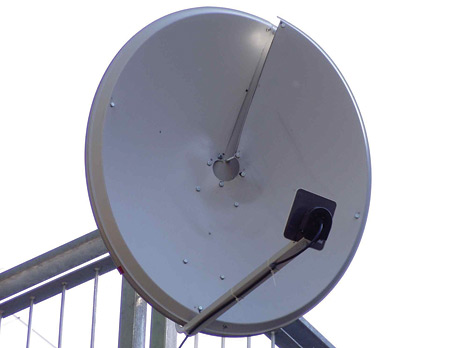
\includegraphics[width=\textwidth]{helical_dish}
	\end{minipage}
	\begin{minipage}{0.49\textwidth}
		\begin{items}
		\item Multiple signals transmitted on the same frequency.
		\end{items}
	\end{minipage}
	
\end{frame}


%\begin{frame}
%
%  \begin{figure}[h]
%    \centering
%    \animategraphics[width=\columnwidth, loop]{10}{anim/test-}{01}{39}
%  \end{figure}
%\end{frame}



\end{document}
